\chapter{Векторні зображення.}\label{cha:vector_images}
Одним із способів описати зображення за допомогою тексту є оголошення його вмісту за допомогою положення та розміру геометричних форм і фігур, таких як лінії, криві, прямокутники та кола;такі зображення називаються \textbf{векторними}.

\begin{figure}
    \label{fig:image3}
    \centering
    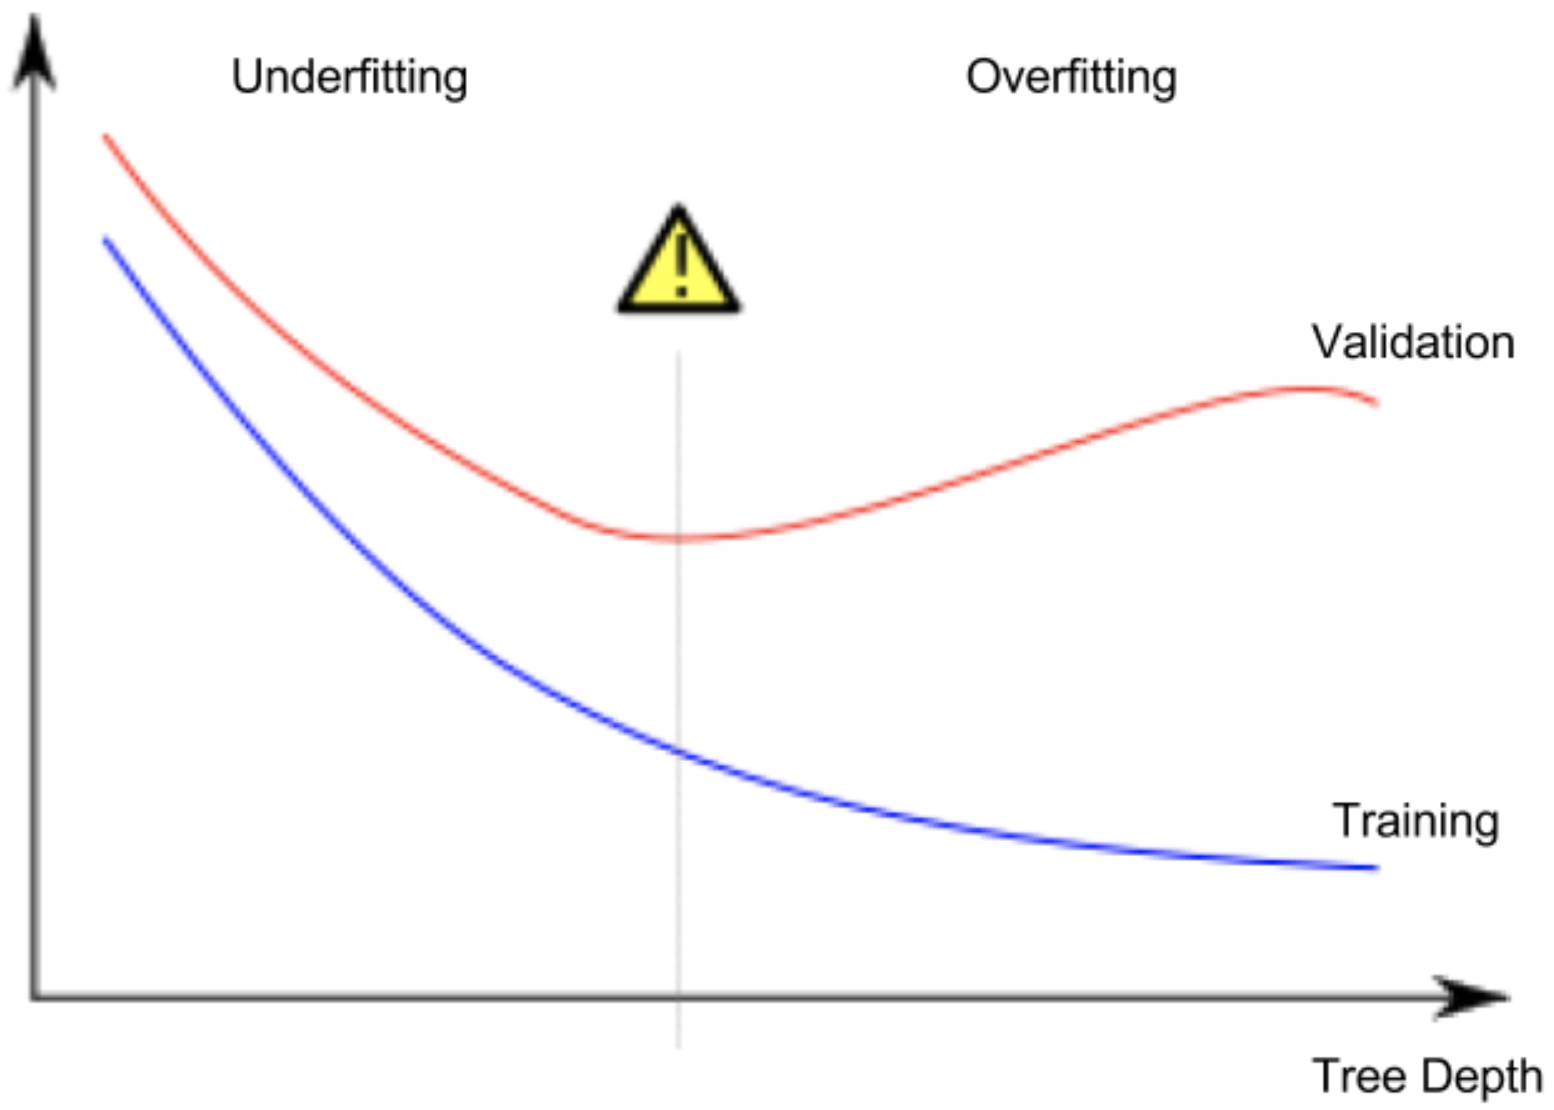
\includegraphics[scale=0.5]{image3.png}

    Рис. 3. Векторне зображення обличчя.
\end{figure}

\begin{lstlisting}[style=light, language=Python,label={lst:vectorimg},caption=Приклад векторного зображення]
            draw circle
                 center        0.5, 0.5
                 radius        0.4
                 fill-color    yellow
                 stroke-color  black
                 stroke-width  0.05
            draw circle
                 center        0.35, 0.4
                 radius        0.05
                 fill-color    black
            draw circle
                 center        0.65, 0.4
                 radius        0.05
                 fill-color    black
            draw line
                 start         0.3, 0.6
                 end           0.7, 0.6
                 stroke-color  black
                 stroke-width  0.1
\end{lstlisting}

\section{Визначаємо форму}\label{sec:defining_shapes}

Попередній опис зображення можна розглядати як "рецепт приготування", як намалювати зображення.
Він містить геометричні примітиви, такі як лінії, криві та кола, що описують колір, а також відносний розмір, положення та форму елементів.
Коли підготовка зображення до відображення повинна бути перетворена у \textbf{растрове зображення}, цей процес називається \textbf{растеризацією}.

Векторне зображення не залежить від роздільної здатності, це означає, що ви можете збільшити або зменшити зображення, не впливаючи на якість виводу.
Векторне зображення не втрачає якість при масштабувані оскільки ми працюємо з декларативним синтаксисом, тобто інструкцією.
Таким чином ми можемо змінювати розмір полотна і не втрачати в якості, оскільки зображення буде пераховане в межах полотна.
Векторні зображення є найкращим способом представлення шрифтів, логотипів та багатьох ілюстрацій.
